%************************************************
\chapter{Introduction}
\label{chp:Introduction}
%************************************************

%\section{Motion Vision}
%what is motion vision. what is the central question we want to answer ? Why do we try to answer above question using drosophila ?

\section{\protect\NoCaseChange{\textit{Drosophila}} as a model organism}
\textit{Drosophila melanogaster} is one of the most powerful model organisms available for the functional dissection of neural circuits. It allows for sophisticated in vivo neural manipulations -- imaging, activation, and suppression of neural activity. The \textit{Drosophila} research community has developed thousands of 'driver-lines' that can be used to express genes of interest in a neuron-specific manner \parencite{Pfeiffer2008}. Along with this, \textit{Drosophila} allows several practical working advantages: They are small, have a short generation time of about 10 days, and are easy to grow in a lab. 

The \textit{Drosophila} brain is estimated to contain about 200,000 neurons \parencite{Raji2021}. It involves computation of modest complexity. These computations are implemented in circuits that contain a limited number of neurons, and with \textit{Drosophila} genetic armoury almost each of these neurons can be precisely targeted. However, even with comparatively little or less complexity, there are surprising parallels between how the fly and mammalian brains process information \parencite{Borst2015}. Insights about the nervous system obtained in \textit{Drosophila} are thus often relevant for other species \parencite{Bellen2010, Venken2011}.

\section{Tools for functional dissection of \protect\NoCaseChange{\textit{Drosophila}} neural circuits}
To have a detailed understanding of how a neural circuit functions, we need to know the role each individual neuron plays in that particular circuit. To achieve this, we would like to perform the following three types of manipulations on the given neuron: (i) record neuronal activity from the neuron, (ii) activate the neuron, and (iii) silence the neuron. Fortunately, years of research in \textit{Drosophila} have provided us with multiple tools in order to be able to perform these manipulations in the choice of neuron we want. The most important tool which enables us to do this in a neuron-specific manner is the Gal4-UAS system (figure \ref{fig:gal4uas}). 

\subsection{GAL4-UAS / LexA-lexAop}
Following the discovery of transposable DNA sequences (P-elements) in the \textit{Drosophila} genome \parencite{Rubin1982}, the GAL4-UAS system was designed \parencite{Brand1993}. The GAL4-UAS system is a binary expression system consisting of two main components: the yeast transcriptional factor GAL4 expressed in a specific pattern and a reporter gene under the control of a UAS promoter that is silent in the absence of GAL4. The Gal4-UAS system essentially involves crossing two fly lines: one called the 'driver-line', defines which neurons express the required effector gene; the other called 'reporter-line', defines what gene is expressed in the neurons defined by the driver line. 

Another independent binary transcriptional system that can be used is the LexA-lexAop system. This method is based on the bacterial DNA-binding operator lexAop and controlled by the expression of LexA. The LexA binds to and activates the lexA operator (lexAop). One can use the LexA-lexAop system in combination with the GAL4-UAS system to simultaneously express genes of interest in two different neuronal populations. %Using a combination of the GAL4-UAS and LexA-lexAop system, one can express the following three types of reporter genes: Indicator, Suppressor \& Activator.
\begin{figure}
\centering
\hspace*{-1cm} 
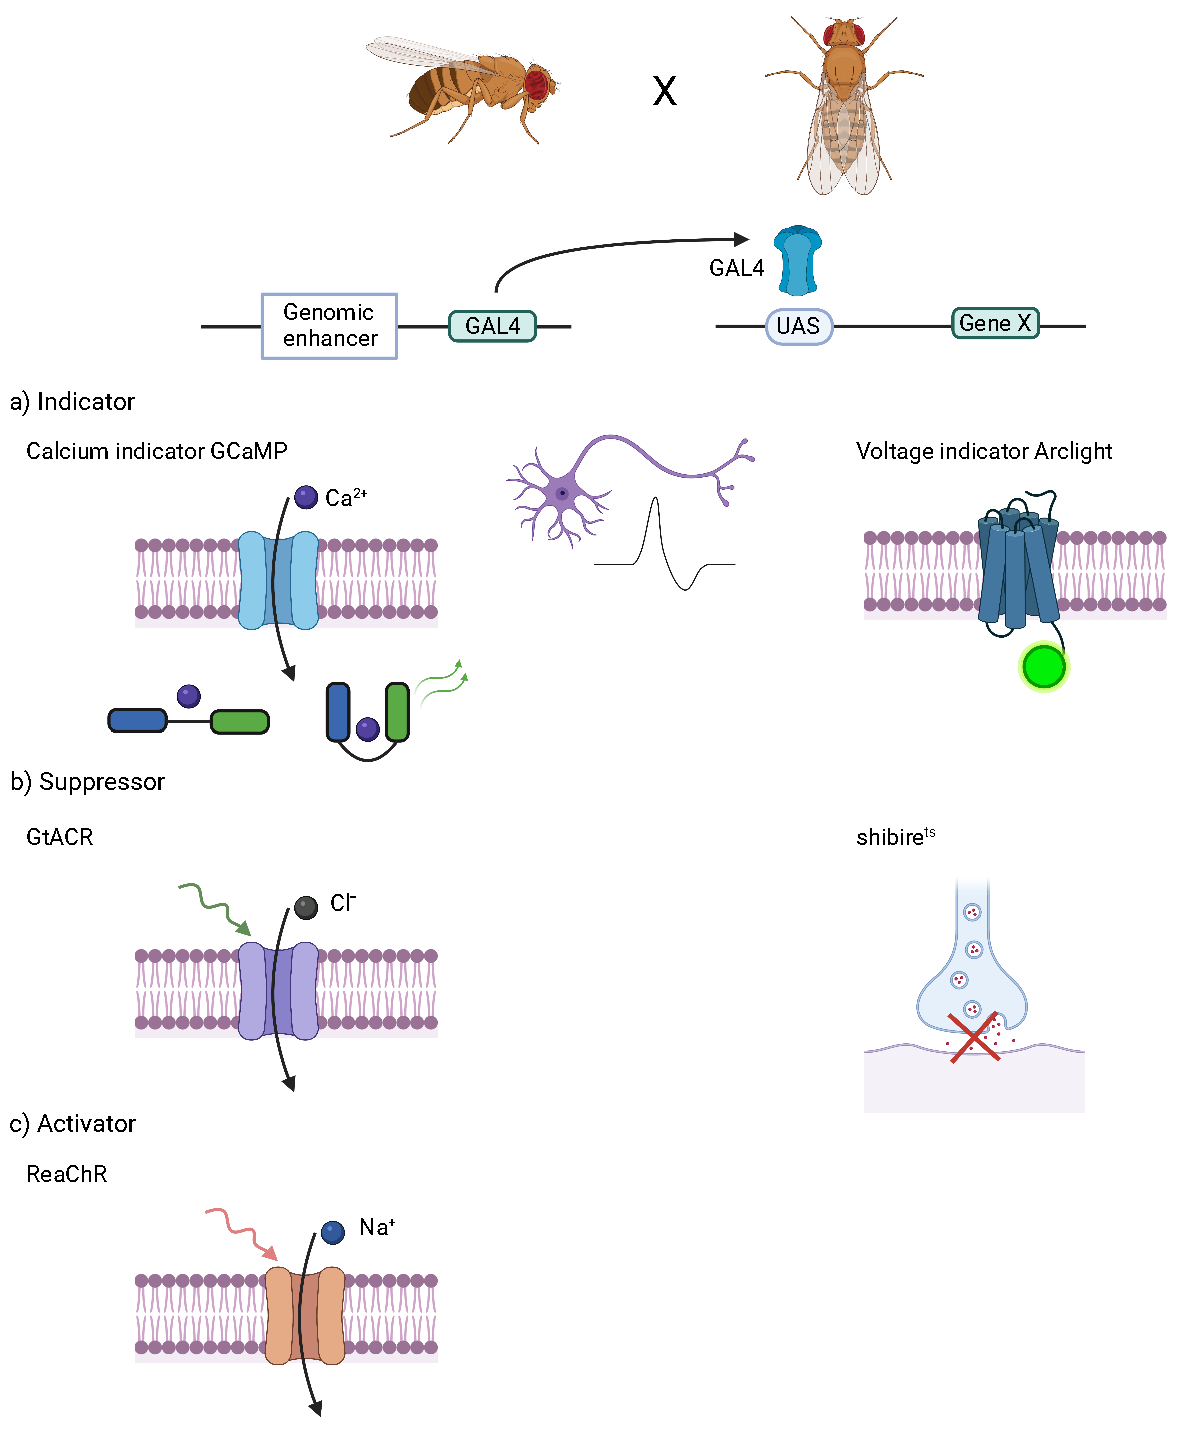
\includegraphics[scale=0.8]{gal4uasfigure}
\caption[Genetic tools for functional manipulations in \textit{Drosophila}] {The Gal4-UAS system is used to express a gene of interest in a specific subset of neurons. (a) The calcium indicator is used to record neural activity using intracellular calcium concentration. The voltage indicator is used to optically record membrane potential changes in the neuron. (b) Neural activity can be suppressed by expressing light-sensitive chloride channels or by blocking synaptic transmission via the expression of temperature-sensitive $shibire^{ts}$. (c) Neurons can be activated via the expression of light-sensitive cation channels. (modified from \cite{Borst2009})}
\label{fig:gal4uas}
\end{figure}
\subsection{Calcium Indicator: GCaMP for recording changes in intracellular calcium}
To record neuronal activity, one can use the GAL4-UAS system to express GFP to visualize a specific neuron type, and then use somatic patch recording to record neural activity from the neuron \parencite{Wilson2004, Joesch2008}. However, neurons in the optic lobe of \textit{Drosophila} are often too small in size for successful electrophysiological recording (but see \cite{Groschner2022, Gruntman2018}). To overcome this, one can use calcium indicators as a proxy for neuronal activity (figure  \ref{fig:gal4uas}a). 

Neural activity causes rapid changes in intracellular free calcium \parencite{Baker1971, Sabatini2002, Egelhaaf1995}. One can thus express genetically encoded calcium indicators (GECIs) which change their fluorescence according to the change in concentration of intracellular calcium. GECIs typically consist of a calcium-binding domain - calmodulin, calmodulin-binding peptide M13, and a reporter element which is based on either a single fluorescent protein or two fluorescent proteins \parencite{Broussard2014}. In the case of a single fluorescent protein for example in GCaMPs, calmodulin (CaM) binds to the M13 peptide in the presence of calcium. This coupling results in conformational changes in the fluorescent protein, resulting in a change in fluorescence intensity \parencite{Nagai2001}. In the case of two fluorescent proteins, conformational changes lead to Förster Resonance Energy Transfer (FRET) between two fluorescent proteins with overlapping excitation and emission spectra \parencite{Miyawaki1997}. In this thesis, we used GCaMP6f  \parencite{Chen2013} in combination with two-photon microscopy for recording neural activity.

%\subsection{Voltage Indicator: Arclight for recording changes in neuronal membrane potential}
%To measure membrane potential changes in neurons, electrophysiology is the most commonly used method. However, single-cell electrophysiological recordings of neurons in the optic lobe have been difficult due to their small size. The evolution of genetically encoded voltage indicators (GEVIs) has made them powerful tools for recording changes in the membrane potentials of neurons \parencite{Yang2016}. Population neuronal activity can be monitored simultaneously and noninvasively using optical methods. GEVIs have a faster temporal resolution compared to the genetically encoded calcium indicators and are a direct readout of voltage changes. Their use in vivo however has been limited by limitations in their dynamic range, brightness, and the ability to be excited by two-photon simulations. Due to the low signal-to-noise ratio, experiments with optical voltage indicators such as ASAP2f have been challenging \parencite{Yang2016}.

%We use a fluorescence protein voltage sensor called Arclight \parencite{Jin2012}. Arclight is based on the fusion of the voltage sensing domain of \textit{Ciona intestinalis} voltage-sensitive phosphatase \parencite{Murata2005} and the fluorescent protein super ecliptic pHluorin with an A227D mutation. Arclight's fluorescence decreases with membrane depolarization and increases with membrane hyperpolarization. We used Arclight in combination with two-photon imaging to record changes in the neuronal membrane potential.

\subsection{Manipulating neural activity}

In order to understand the principles of information processing in a neural circuit, along with recording neural activity we would also like to either suppress or activate neural activity in specific neurons in the circuit. Inactivation and activation of genetically defined cell types helps to establish causal relations in a specific group of neurons and neural circuits. There are several tools that allow for the inactivation of a neuron. Cell death genes such as \textit{reaper (rpr)} and \textit{head involution defective (hid)} or \textit{grim} induce apoptosis \parencite{Chen1996, Grether1995}.  The tetanus toxin light chain cleaves the synaptic vesicle protein synaptobrevin and inhibits neurotransmitter exocytosis at chemical synapses \parencite{Sweeney1995}. The expression of Kir -- an inwardly rectified potassium channel, causes neurons to hyperpolarize, resulting in suppressed excitability \parencite{Johns1999}. %While using the Gal4-UAS system to express these effectors provides effective control over the functionality of the targeted neurons, it also creates some unwanted problems. First, because most enhancers are active at several stages of development, it is difficult to avoid the toxic effects of the expressed gene products on development. Second, if particular neurons are eliminated during development, their loss in function may be compensated by some other neuron, hence making interpretation of results difficult. Third, it is not possible to observe acute effects elicited by the temporal inactivation of particular neurons. To overcome these limitations, we can use the conditional effector proteins like $shibire^{ts}$ \& GtACR (figure  \ref{fig:gal4uas}b), which is activated by higher temperature and light respectively. 

\textit{Drosophila shibire} encodes the protein dynamin, which is involved in the process of endocytosis and is essential for vesicle recycling. The dominant-negative temperature-sensitive allele $shibire^{ts}$ is defective in synaptic vesicle recycling at the restrictive temperature ($>29\degree C$) which results in rapid and reversible inhibition of synaptic transmission \parencite{Kitamoto2001}. \cite{Joesch2010} showed that flies expressing $shibire^{ts}$ if exposed to persistent heat-shock for one hour at restrictive temperature $(37\degree C)$, the output of affected cells is suppressed for several hours. This experimental method gives us a longer time duration, which allows us to record neural activity from the fly while the activity from the neuron expressing $shibire^{ts}$ is suppressed. However, we get this extra time duration at the cost of losing the reversibility of the intervention.

The tools mentioned above allow for cell-type-specific silencing. However, in addition to the cell-type-specificity, we would also like to have temporally accurate and reversible silencing. \textit{Guillardia theta} Anion Channel Rhodopsins (GtACR1 and GtACR2) can provide us with these additional advantages \parencite{Govorunova2015}. GtACRs impart strong light-gated chloride conductance and is much more light-sensitive than the Halo-\\rhodopsin class of chloride pumps. In particular, in the fly visual system, GtACR1 can be used since its activation spectrum is shifted towards longer wavelengths with respect to five of the six \textit{Drosophila} rhodopsins (except rhodopsin 6) \parencite{Mauss2017, Mohammad2017}. %Thus, we can use the Gal4-UAS system to express GtACR in neurons we want to hyperpolarize and silence the neural activity. Simultaneously, we can express GCaMP in downstream neurons using the LexA-lexAop system and record their neural activity, while silencing the neurons expressing GtACR. 
 
%\subsection{Activator: ReaChr for activating neuron}
Along with using GCaMP for imaging, $shibire^{ts}$ or GtACR for suppressing neural activity, we would also like to have a tool for activating neurons. An ideal method for activation requires excellent temporal control. Light-gated cation channels - Channelrhodopsins(ChRs) can be used for this purpose (figure  \ref{fig:gal4uas}c). ChRs are light-gated, non-specific cation channels that allow selective depolarization of genetically targeted cells \parencite{Lin2013, Busch2018}. 

%Therefore by combining the use of GCaMP for calcium imaging and GtACR for suppression or ReaChR for activation, we can better understand the functions of neurons present in a given neural circuit.
\section{Physiological techniques for recording neural activity}
In order to understand neuronal signaling and how signals propagate between neurons, it is necessary to record neural activity. Whole-cell patch clamp recording and two-photon imaging are the most commonly used methods in \textit{Drosophila melanogaster}.

\subsection{Whole-cell patch clamp recording}
Electrophysiological recording can be used to measure neural activity in vivo with a high temporal resolution. For \textit{Calliphora}, different recording techniques have been established, including extracellular recordings and sharp electrode intracellular recordings \parencite{Haag2001, Laughlin1989, Bishop1967}. Due to the small size of many neurons in \textit{Drosophila}, electrophysiological recordings in \textit{Drosophila melanogaster} were only established in the last two decades. Recordings with sharp electrodes was not possible because of the small size of the neurons in \textit{Drosophila}. A slightly different method, known as whole-cell patch-clamp recording, was developed \parencite{Sakmann1984}. Whole-cell patch clamp recording was used to record from tangential cells in the \textit{Drosophila} \parencite{ Joesch2008}. Patch clamp recordings of whole cells are limited mainly by two factors: the size of neurons and their anatomical accessibility. In spite of this, different brain regions were successfully recorded \parencite{Behnia2014, Murthy2008, Wilson2004}. Currently, even neurons with very small soma size ($\approx 2-3 \, \mu m$) like T4/T5 and medullary neurons can be recorded \parencite{Gruntman2018, Groschner2022}.

\subsection{Two-photon imaging}
In many areas of natural science, including neuroscience, two-photon imaging \parencite{Denk1990} has been a milestone. Despite the fact that electrophysiological methods can collect high-resolution data ($\approx 10kHz$), they are not capable of recording from large populations of neurons. Two-photon imaging can be used in such cases. Additionally, two-photon imaging is non-invasive.The two-photon imaging technique combines laser scanning fluorescence microscopy with functional reporters like GCaMP to detect neuronal activity. Fluorescence proteins are stimulated using a femtosecond-pulsed laser of twice the wavelength of the reporters excitation spectrum peak ($\approx 900 \, nm$ for GCaMP). It takes two coinciding photons to overcome the threshold of excitation because a single photon lacks the energy necessary to excite the fluorophore. As a result, fluorescence is spatially restricted to the laser stimulation focus point. In addition, the laser's high wavelength is beyond the range of the spectral sensitivity of \textit{Drosophila}'s photoreceptors. Therefore, two-photon imaging is suitable for investigating the response properties of neurons within the visual system \parencite{Maisak2013, Reiff2010, Strother2018}.

\section{Neural communication}
Camillo Golgi's silver-stain method made it possible to visualize the nervous system in tissue samples under the light microscope (1873). Santiago Ramón y Cajal in 1888 described the nervous system as a network of individual cells. About a decade later, in 1897, the term 'synapse', derived from the Greek word 'synapsis' (meaning 'conjunction'), was used to describe the connections between two neurons. Neurons form networks where they communicate via synapses. Two types of synapses exist 1) electrical synapses and 2) chemical synapses.

\subsection{Electrical synapses}
In electrical synapses, two cells are directly connected by a cluster of intercellular channels called gap junctions \parencite{Bennett2004}. The gap junctions provide a conductive pathway for electrical current to spread between cells that are interconnected. Consequently, electrical currents underlying action potentials or graded potentials directly propagate to postsynaptic neurons, with a similar time course to presynaptic signals. Additionally, since electrical signals propagate bidirectionally, signalling events generated in the postsynaptic cells also spread to the presynaptic cells. In \textit{Drosophila}, electrical synapses are widely distributed throughout the nervous system and are essential to neuronal function \parencite{Ammer2022, Stebbings2002, Liu2016}.

%In order to guide animal behavior, neurons perform a wide range of computations. Neurons encode information via graded changes in membrane potential or action potential frequency.


\subsection{Chemical synapses}
Neurons communicate mostly via chemical synapses (figure  \ref{fig:chemicalsynapse}) which require the release of neurotransmitters. When the presynaptic membrane is sufficiently depolarized, voltage-gated calcium channels open and allow $Ca^{2+}$ to enter the cell \parencite{Luo2020}. Calcium entry leads to the fusion of synaptic vesicles with the membrane and the release of neurotransmitter molecules into the synaptic cleft \parencite{Chapman2002}.  As neurotransmitters diffuse across the synaptic cleft, they bind to receptors in the postsynaptic membrane, causing the postsynaptic neuron to depolarize or hyperpolarize, thereby passing the information from pre to postsynaptic neurons \parencite{Maio2008}. Calcium plays a critical role in the release of neurotransmitters. Voltage-to-calcium transformation in neurons is therefore a crucial step in neural information processing and neural computation. 

\begin{figure}
\centering
\hspace*{-1cm} 
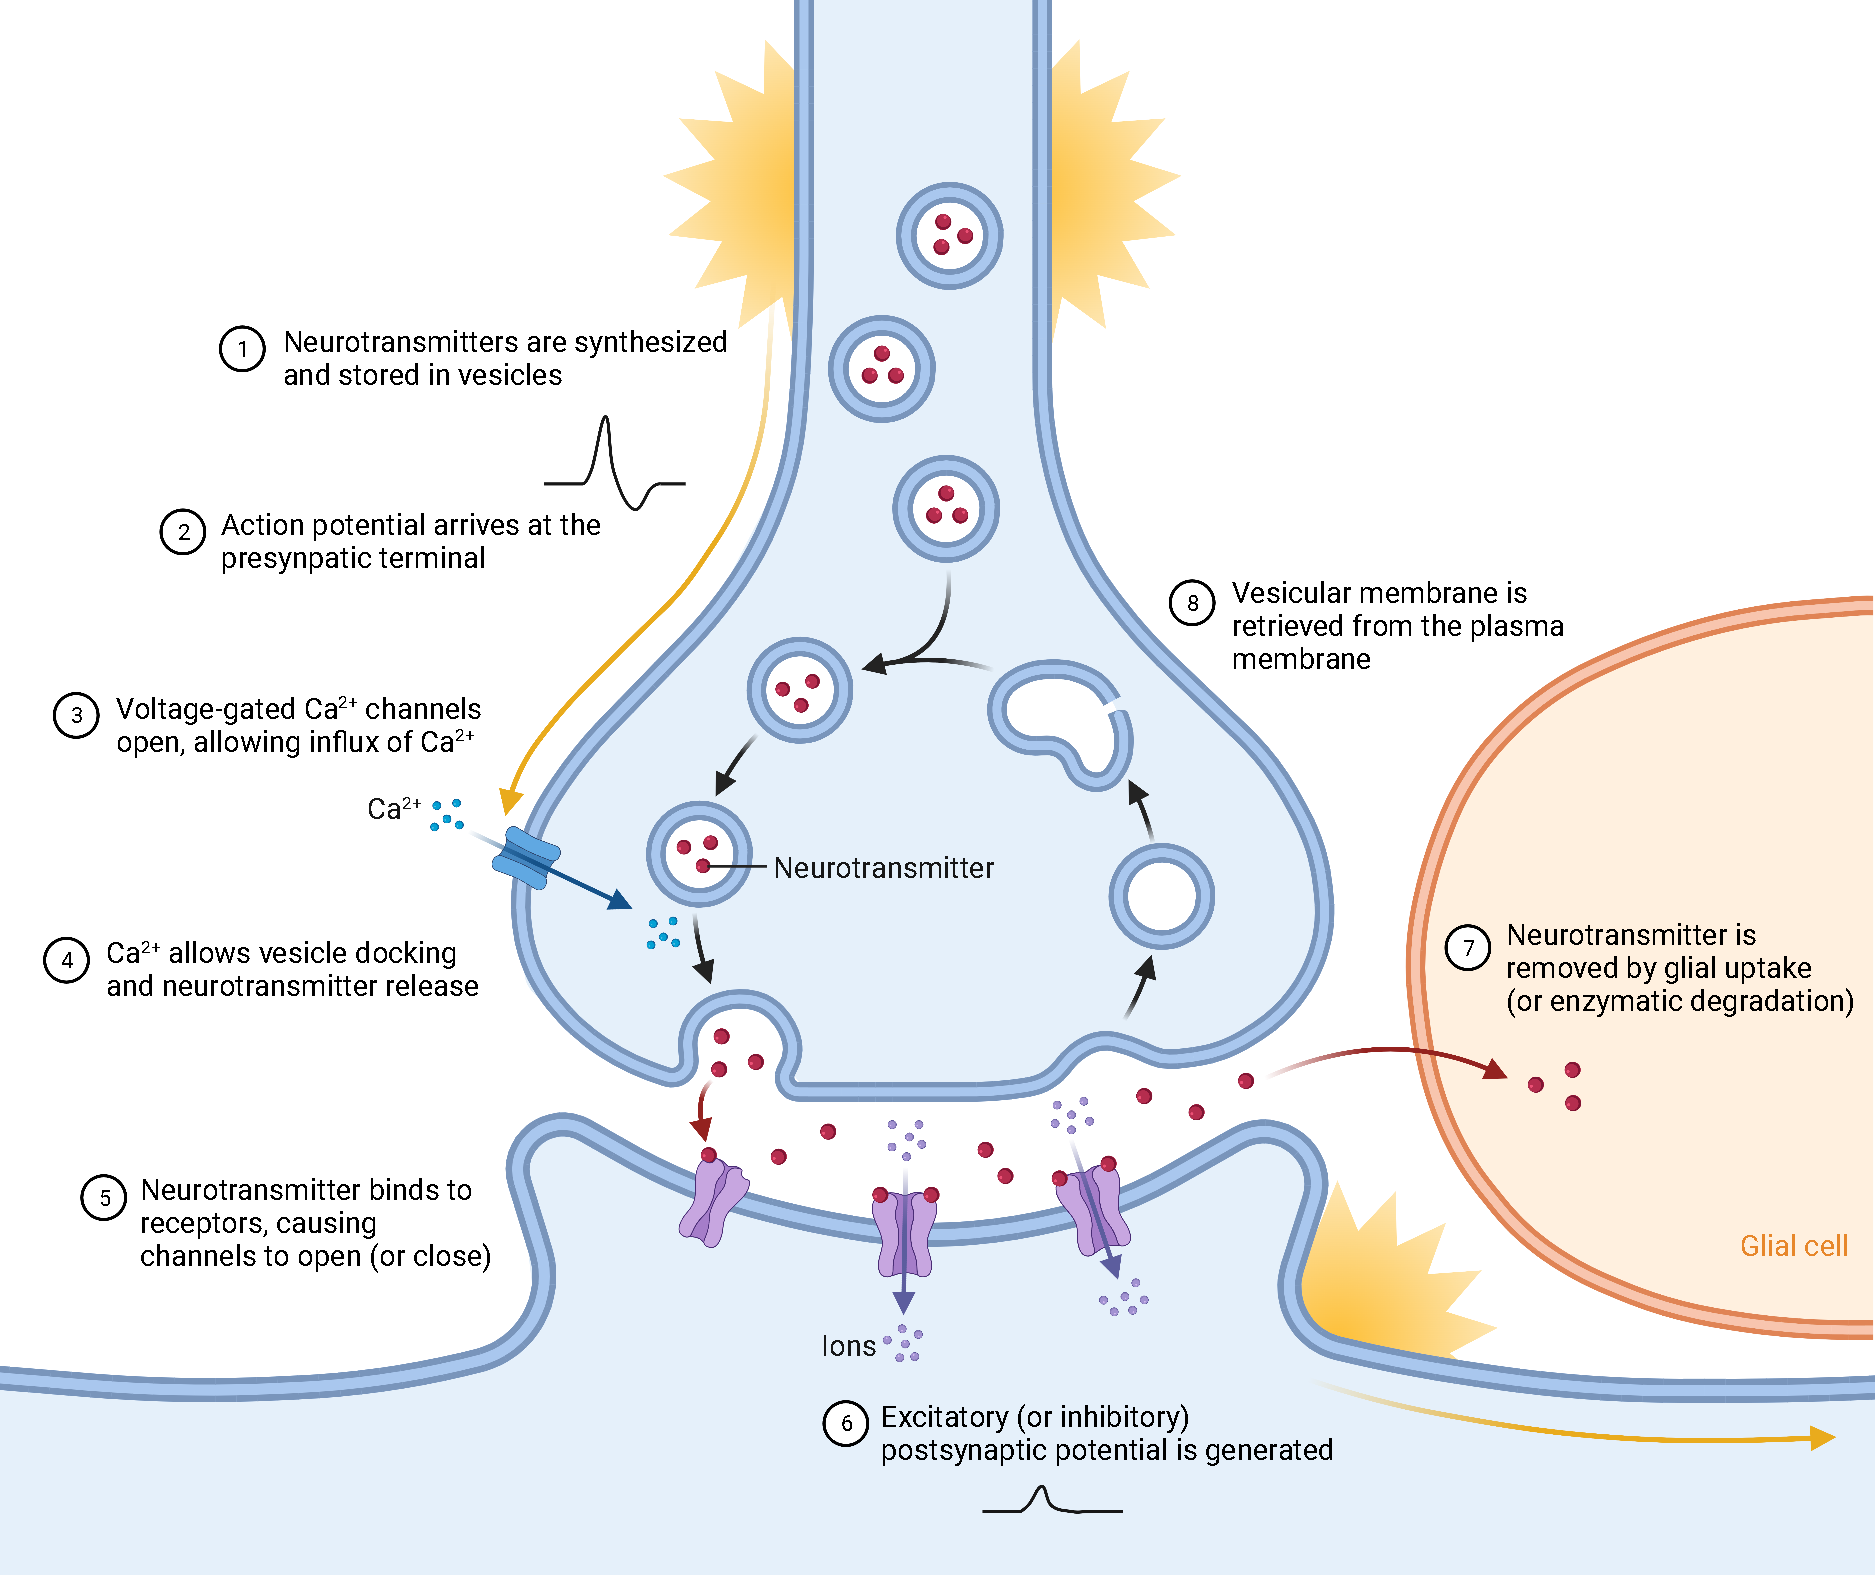
\includegraphics[scale=0.45]{Chemical_Synapse}
\caption[Chemical synapse: steps of synaptic transmission] {Chemical synapse: steps of synaptic transmission. (1) Synthesis and storage of neurotransmitters in the vesicles. (2) Depolarization in the presynaptic terminal causes (3) voltage-gated calcium channels to open and allow an influx of calcium ions. (4) High concentration of calcium ions triggers the fusion of neurotransmitters-filled vesicles with the presynaptic membrane and the release of neurotransmitters into the synaptic cleft. (5) Neurotransmitters released in the synaptic cleft bind to receptors in the postsynaptic membrane leading to (6) excitatory or inhibitory postsynaptic potential. (figure created with \href{https://app.biorender.com/biorender-templates}{Biorender.com})}
\label{fig:chemicalsynapse}
\end{figure}

\subsection{Voltage-gated ion channels}
Voltage-gated ion channels are transmembrane proteins that allow certain inorganic ions to cross cell membranes (figure  \ref{fig:vgatedionc}). Generally, these channels consist of two distinct but functionally coupled transmembrane domains: the voltage sensing domain and the pore domain. The voltage sensing domain changes the conformation of the pore domain in response to the changes in transmembrane potential, allowing selected ions to flow down their electrochemical gradient. 

\paragraph{Voltage-gated calcium channels}
Voltage-gated calcium channels mediate depolarization-induced calcium influx that drives the release of neurotransmitters. The $\alpha1$-subunit of the voltage-gated calcium channels forms the ion-conducting pore, which makes it distinct from other calcium channels. Three families of genes encode $\alpha1$ subunits. \textit{Drosophila} genome has one $\alpha1$ subunit gene in each family: $\alpha1D$ ($Ca_{v}1$), cac ($Ca_{v}2$), and $\alpha1T$ ($Ca_{v}3$) \parencite{Littleton2000, King2007}. In \textit{Drosophila} antennal lobe projection neurons, cac ($Ca_{v}2$) type and $\alpha1T$ ($Ca_{v}3$) type voltage-gated calcium channels are involved in sustained and transient calcium currents, respectively \parencite{Gu2009, Iniguez2013}.

\paragraph{Voltage-gated sodium channels}
In neurons, voltage-gated sodium channels play a crucial role in the initiation and propagation of action potentials \parencite{Hodgkin1952}. Sodium channels are activated and deactivated within milliseconds when the membrane is depolarized by a few millivolts. There are at least ten genes in mammals that encode these large membrane proteins. In contrast, \textit{paralytic (para)} is the only voltage-gated sodium channel gene described in Drosophila \parencite{Piggott2019}. %Loss of \textit{paralytic (para)} reduces neuroblast progeny cell number in \textit{Drosophila} \parencite{Piggott2019}.

\paragraph{Voltage-gated potassium channels}
Voltage-gated potassium channels are transmembrane channels specific to potassium ions. They play a crucial role in returning the depolarized cell to its resting membrane potential, after each action potential. Voltage-gated potassium channels are the most diverse family of voltage-gated ion channels in the human genome, with 40 members for $\alpha$ subunit grouped into 12 families \parencite{Gutman2005}. The first voltage-gated potassium channel discovered in the \textit{Drosophila} was \textit{Shaker} \parencite{Papazian1987}. Afterwards, three additional \textit{Shaker} like voltage-gated potassium genes were identified in \textit{Drosophila}: \textit{Shab}, \textit{Shaw} and \textit{Shal} \parencite{Covarrubias1991}. 

\begin{figure}
\centering
\hspace*{-1cm} 
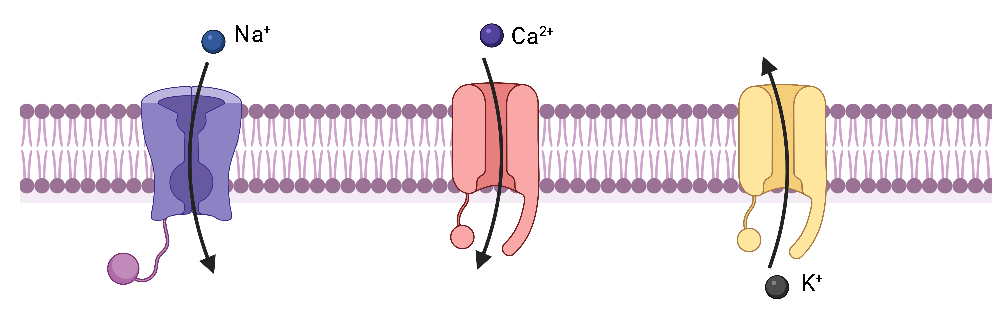
\includegraphics[scale=0.85]{voltagegatedionchannels}
\caption[Voltage-gated ion channels] {Voltage-gated ion channels: The sodium channels allow $Na^{+}$ ions to enter the cell. The calcium channels allow $Ca^{2+}$ ions to enter the cell. The potassium channels allow efflux of the $K^{+}$ ions.}
\label{fig:vgatedionc}
\end{figure}


\section{Fly motion vision system}
The \textit{Drosophila} visual processing pathway is comprised of retina, lamina, medulla, lobula and lobula plate, each arranged in a columnar, retinotopic fashion (figure \ref{fig:opticlobe}a) \parencite{Fischbach1989}. Each compound eye contains around 750 ommatidia \parencite{Ready1976}. The ommatidia of each eye are arranged in a regular lattice with a 5-degree inter-ommatidia angle \parencite{Land1997}. There are eight different photoreceptors in each ommatidium (R1-R8). A circular arrangement is formed by R1-R6 enclosing R7 and R8, which are stacked on top of one another. Rhodopsin 1 (Rh1), which detects a wide range of light wavelengths, is expressed in R1-R6. Peak sensitivity for Rh1 occurs at two distant locations in the light spectrum: one near 480 nm (e.g. green light) and one at UV wavelengths. Motion detection is impaired without this pigment \parencite{Rister2007}. Different types of rhodopsins are expressed in R7 and R8, with distinct absorption peaks suitable for color vision and polarized light detection \parencite{Yamaguchi2008, Wernet2004}.

\paragraph{Retina and Phototransduction}
Since R1-R6 are arranged in a circular pattern in each ommatidium, each photoreceptor collects light from a slightly offset position. Fly eyes are curved, however, so certain photoreceptors of adjacent columns have the same optical axis. Hence, seven photoreceptors of seven different ommatidia receive light at the same position in the fly's eye due to its hexagonal structure. Consequently, the seven photoreceptors' inputs converge downstream in one lamina cartridge, increasing visual sensitivity without compromising spatial resolution. It is known as neural superposition \parencite{Kirschfeld1967}.

Phototransduction is the process of converting photons into electrical signals. A G-protein-coupled signaling cascade is involved in the phototransduction in \textit{Drosophila melanogaster}, as in most invertebrates \parencite{Hardie2015}. Light-guiding rhabdomeres, which contain approximately 30,000 microvilli, are responsible for this process \parencite{Hardie2001}. Rhodopsins are membrane-bound pigments that are part of the signaling cascade contained within each microvillus. The chromophore 11-cis-3-hydroxy-retinal is covalently bound to these G-protein-coupled receptors. The chromophore is converted to all-trans-retinal upon photon absorption. As a result of this conversion, rhodopsin undergoes a conformational change into metarhodopsin, which serves as a catalyst for the activation of heterotrimeric G-proteins. As a result, phospholipase C (PLC) is activated, resulting in the activation of cation-permeable channels via a variety of potential mechanisms, and depolarizing the photoreceptors, ultimately leading to the release of inhibitory neurotransmitter histamine \parencite{Hardie2001}. Invertebrates can directly reisomerize metarhodopsin to rhodopsin simply by absorbing longer wavelength light. In vertebrate phototransduction, all-trans-retinal must be re-isomerized in a slow enzymatic process. Long-wavelength light can pass through the screening pigment, enabling rapid switching between the two states. As a result, longer wavelength light is trapped and can continuously reset the transduction cascade \parencite{Hardie2001}. Mutations within the signaling cascade can also result in significant visual deficits and blindness \parencite{Hardie2012}.

\begin{figure}
\centering
\hspace*{-1cm} 
\includegraphics[scale=0.75]{fly_optic_lobe}
\caption[Fly optic lobe] {Fly optic lobe: (a) The horizontal cross-section of a reduced silver stain shows the columnar organization of the retina (R), lamina (L), external chiasm (EC), medulla (M), internal chiasm (IC), lobula (Lo), and lobula plate (Lp). Scale bar = $50 \, \mu m$. Reproduced, with permission, from \cite{Takemura2008} (b) Schematic illustration of direction selectivity: moving a bar in front of a fly's eye leads to depolarization of photoreceptors every time, regardless of whether the bar moves to the right or left. It is a non-directional signal. A few synapses downstream, on the lobula plate tangential cells, signals are direction-selective: these cells depolarize during movement along one direction, i.e., their 'preferred' direction, and hyperpolarize during motion along the opposite direction, i.e., their 'null' direction. (c) An overview of all types of columnar cells in the \textit{Drosophila} optic lobe. (\cite{Fischbach1989}) (d) Columnar cell types involved in the motion vision circuit. (Used with permission from \cite{Borst2020, Borst2020b})}
\label{fig:opticlobe}
\end{figure}

\paragraph{Lamina}
The lamina is organized in an array of ${\approx}750$ retinotopic columns (also called 'cartridges'). Each column corresponds to ${\approx}5\degree$ discrete sample of the visual world. The light-sensitive photoreceptors, R1-6 project their axons into each lamina column. Two other photoreceptors, R7 \& R8 pass through the lamina and synapse in specific layers of the medulla. Along with photoreceptor axons, the lamina includes 5 lamina output neurons (L1-L5), six putative feedback neurons (T1, Lat, Law1, Law2, C2, C3), and one lamina intrinsic neuron (Lai). The lamina columnar monopolar neurons, L1-L5 send their axonal projections into specific layers of the medulla. \parencite{Fischbach1989, Tuthill2013}. Lamina output neurons L1 and L2 are the primary input cells for motion vision \parencite{Zhu2013}.


\paragraph{Medulla}
Lamina cells send input projections to the medulla, the second neuropil in the optic lobe. In the medulla, there are ten synaptic layers (M1 to M10) composed of over 60 types of cells. The medulla is composed of hexagonal columns, similar to the lamina. In this way, the mapping between lamina and medulla remains retinotopic. The fibers connecting lamina to medulla form a chiasm, in which posterior medulla cartridges receive input from anterior lamina cartridges. The medulla neurons can be clustered into different groups based on their anatomy and projections. Medulla intrinsic ('Mi') neurons connect different layers of the medulla to each other. Trans-medulla ('Tm') neurons connect specific layers of the medulla to various layers in the lobula. The Trans-medulla Y ('TmY') neurons connect specific layers of the medulla to various layers in the lobula and lobula plate. The direction-selective cell T4 connects medulla layer 10 to the four layers of the lobula plate.

\paragraph{Lobula}
There are at least six layers in the lobula \parencite{Fischbach1989}. Lobula columnar (LC) neurons receive major inputs from the medulla and are the most prominent type of cell in the lobula. Multiple types of LC neurons span the entire visual field in a retinotopic manner \parencite{Otsuna2006}. In total, these neurons are divided into more than twenty distinct subtypes, each conveying information about a different visual feature \parencite{Wu2016}. The direction-selective cell type T5 connects first lobula layer to the four layers of the lobula plate.

\paragraph{Lobula Plate}
There are four layers in the lobula plate, each containing lobula plate tangential cells (LPTCs). Dendritic trees of the LPTC span large areas of the lobula plate, sometimes covering the entire layer. Thus, their receptive fields cover a large portion of the visual field. The neurons that make up this group are composed of more than 60 different types, and they form a complex network of electrical and chemical synaptic connections that form a dense network \parencite{Borst2010}. According to their response characteristics, \textit{Drosophila's} LPTCs can be classified into two major groups: horizontal system cells (HS) and vertical system cells (VS). There are at least three HS cell types (south, equatorial, and north: HS-N, HS-E, HS-S) and six VS cell types (plus three VS-like cells), as well as dorsal and ventral centrifugal horizontal (dCH and vCH) cells in the fruit fly. There is a layer-specific dendritic stratification in the lobula plate, some samples consisting of more than 100 columns. For instance, HS cells mainly receive input from layer 1, processing horizontal motion information. However, VS cells mainly ramify in layer 4 (although some also stratify to other layers) and process vertical motion data.

If one were to record from a single photoreceptor in the retina, it would show a similar response to moving images irrespective of the direction of motion: meaning it is not direction-selective. However, if one records around 4 synapses downstream, Lobula Plate Tangential Cells (LPTCs) depolarise in response to the image moving in its preferred direction and hyperpolarize if the image moves in the opposite direction or the null direction (figure \ref{fig:opticlobe}b). HS (Horizontal System) cells for example are responsive to horizontal motion \parencite{Schnell2010}, while VS (Vertical System) cells are responsive to vertical motion \parencite{Joesch2008}. LPTCs however, integrate over large parts of visual fields, i.e. they are not local motion detectors. Hence, the question arises: which cells are the local motion detectors? 

The answer to the above question is: T4 and T5 are the first local motion detectors found in the \textit{Drosophila} ON and OFF motion vision pathway, respectively. Four sub-population of T4a-d and T5a-d cells tuned to the four cardinal directions and projecting to the four layers in the lobula plate can be found within each column \parencite{Maisak2013}. This leads to the next question: what makes T4 and T5 direction selective? To answer this question, we need to investigate the cells which are present between the non-direction-selective photoreceptors in the retina and direction-selective T4, and T5 cells in Medulla and Lobula respectively (figure \ref{fig:opticlobe}c, d). The columnar cell types of the lamina, medulla, lobula, and lobula plate have been identified and described \parencite{Fischbach1989, RamonyCajal1915}.  

While the cell types were known, the small size of these neurons made electrophysiological recordings difficult. Only after the advent of modern two-photon imaging in combination with using the Gal4-UAS system to express GCaMP in these cells, has it become possible to record neuronal activity from these cells. Experiments over the years revealed the following interesting results : (a) Visual processing in \textit{Drosophila} occurs in two parallel processing pathways for luminance increment (ON) and brightness decrement (OFF) \parencite{Joesch2010, Joesch2013, Strother2014, Eichner2011, Behnia2014, Shinomiya2014} (b) T4 and T5 are first local motion detectors found in the \textit{Drosophila} ON \& OFF motion vision pathway respectively. Four sub-population of T4a-d and T5a-d cells tuned to the four cardinal directions and projecting to the four layers in the lobula plate can be found within each column \parencite{Maisak2013}. 


\subsection{Parallel ON and OFF processing pathways}
In striking similarity to the mammalian retina \parencite{Masland2012}, visual processing in \textit{Drosophila} occurs in two parallel ON and OFF processing pathways \parencite{Borst2015}. The ON pathway transmits information about brightness increments, while the OFF pathway transmits information about brightness decrements. In order to understand the split of photoreceptor (R1-R6) signals into ON and OFF pathways, studies have been done blocking Laminar monopolar cells, while simultaneously recording from downstream LPTCs neurons. While blocking L1 neurons resulted in a specific reduction of LPTC's response to ON stimulus (brightness increment), blocking L2 neurons resulted in a specific reduction of LPTC's response to OFF stimulus (brightness decrement) \parencite{Joesch2010}. In behavioral experiments, walking flies were unable to follow either ON or OFF motion when either L1 or L2 was blocked respectively \parencite{Clark2011}. The flies become completely motion-blind if both L1 and L2 are permanently hyperpolarized (via Kir) \parencite{Tuthill2013, Bahl2013}. These experiments together suggest that the L1 pathway specifically transmits information about brightness increments to the downstream ON motion detector, and the L2 pathway specifically transmits information about brightness decrements to the downstream OFF motion detector. 

\subsection{T4 and T5 cells}
Based on previous studies from \parencite{Fischbach1989, Buchner1984}, T4 and T5 were long thought to be the prime candidates for local motion detectors in the ON and OFF pathways respectively. However, due to its small size, it was difficult to do electrophysiological recordings from T4 and T5 cells \parencite{Douglass1996}. This problem was solved using a combination of 2-photon imaging and a Gal4-UAS system to express GCaMP in T4, and T5 cells to record its neural activity in response to the ON and OFF stimuli. Stimulating the flies with visual motion in four cardinal directions (front-back, back-front, upwards, and downwards), \cite{Maisak2013} recorded direction-selective activity from T4/T5 cells. Four sub-populations of T4a-d and T5a-d cells tuned to the four cardinal directions and projecting to the four layers in the lobula plate were found within each column. Further, the T4 cells were found to respond specifically to ON stimulus and the T5 cells were found to respond specifically to OFF stimulus. Blocking T4 and T5 cells led to a complete loss of motion response in the lobula plate tangential cells \parencite{Schnell2012}, and of the optomotor response of tethered walking flies \parencite{Bahl2013}. Specific blocking of T4 cells led to a reduction in LPTC and optomotor responses to ON stimulus selectively, while specific blocking of T5 cells led to a reduction in LPTC and optomotor responses to OFF stimulus selectively. These results together suggest T4 and T5 cells to be the elementary motion detector for the ON and OFF pathways respectively \parencite{Maisak2013}.      

\section{Neural circuit underlying direction selectivity}
Having identified T4 and T5 cells as the elementary local motion detectors, the next question which arises is which cells provide synaptic inputs to T4 and T5 cells. Electron Microscopy (EM) studies \parencite{Shinomiya2019, Takemura2017} provided the answer to this question. \cite{Shinomiya2019} used FIB-SEM (Focused Ion Beam Scanning Electron Microscopy) to record a volume of the optic lobe comprising seven columns of the medulla, lobula, and lobula plate. They identified all the different neuron types providing inputs to the T4 and T5 cells. T4 cells receive input from Mi1, Tm3, Mi4, Mi9, C3, CT1, and TmY15. T5 cells receive input from Tm1, Tm2, Tm4, Tm9, CT1, TmY15, LT33, and Tm23. The T4 and T5 cells' dendrites span several columns along the preferred direction of the motion. The authors could also locate where the different cell types synapse onto the dendrites of T4 and T5. For example, a T4c cell with the preferred direction of motion as upwards receives input from Mi1, Tm3, and TmY15 in the central part of its dendrite, from Mi9 and T4c on the ventral part, and from Mi4, C3, and CT1 on the dorsal part of its dendrite [figure \ref{fig:t4t5inputsynapses} top]. T4d cells with preferred direction as downwards receive input from Mi1, Tm3, and TmY15 in the central part, from Mi9 and T4d on the dorsal part, and from Mi4, C3, CT1 on the ventral part of its dendrite. In summary, all T4 subtypes receive inputs from Mi1, Tm3, and TmY15 in the central part, from Mi9 on the preferred side (i.e. the side from which a preferred direction stimulus approaches), and from Mi4, C3, and CT1 on the null side (i.e. the side from which a null direction stimulus approaches) of their dendrite. Similarly, all T5 subtypes receive inputs from Tm1, Tm2, and Tm4 on the central part, Tm9 on the preferred side, and CT1 on the null side of their dendrite [figure \ref{fig:t4t5inputsynapses}]. %a figure showing summary of different inputs.    

\begin{figure}
\centering
\hspace*{-1.4cm} 
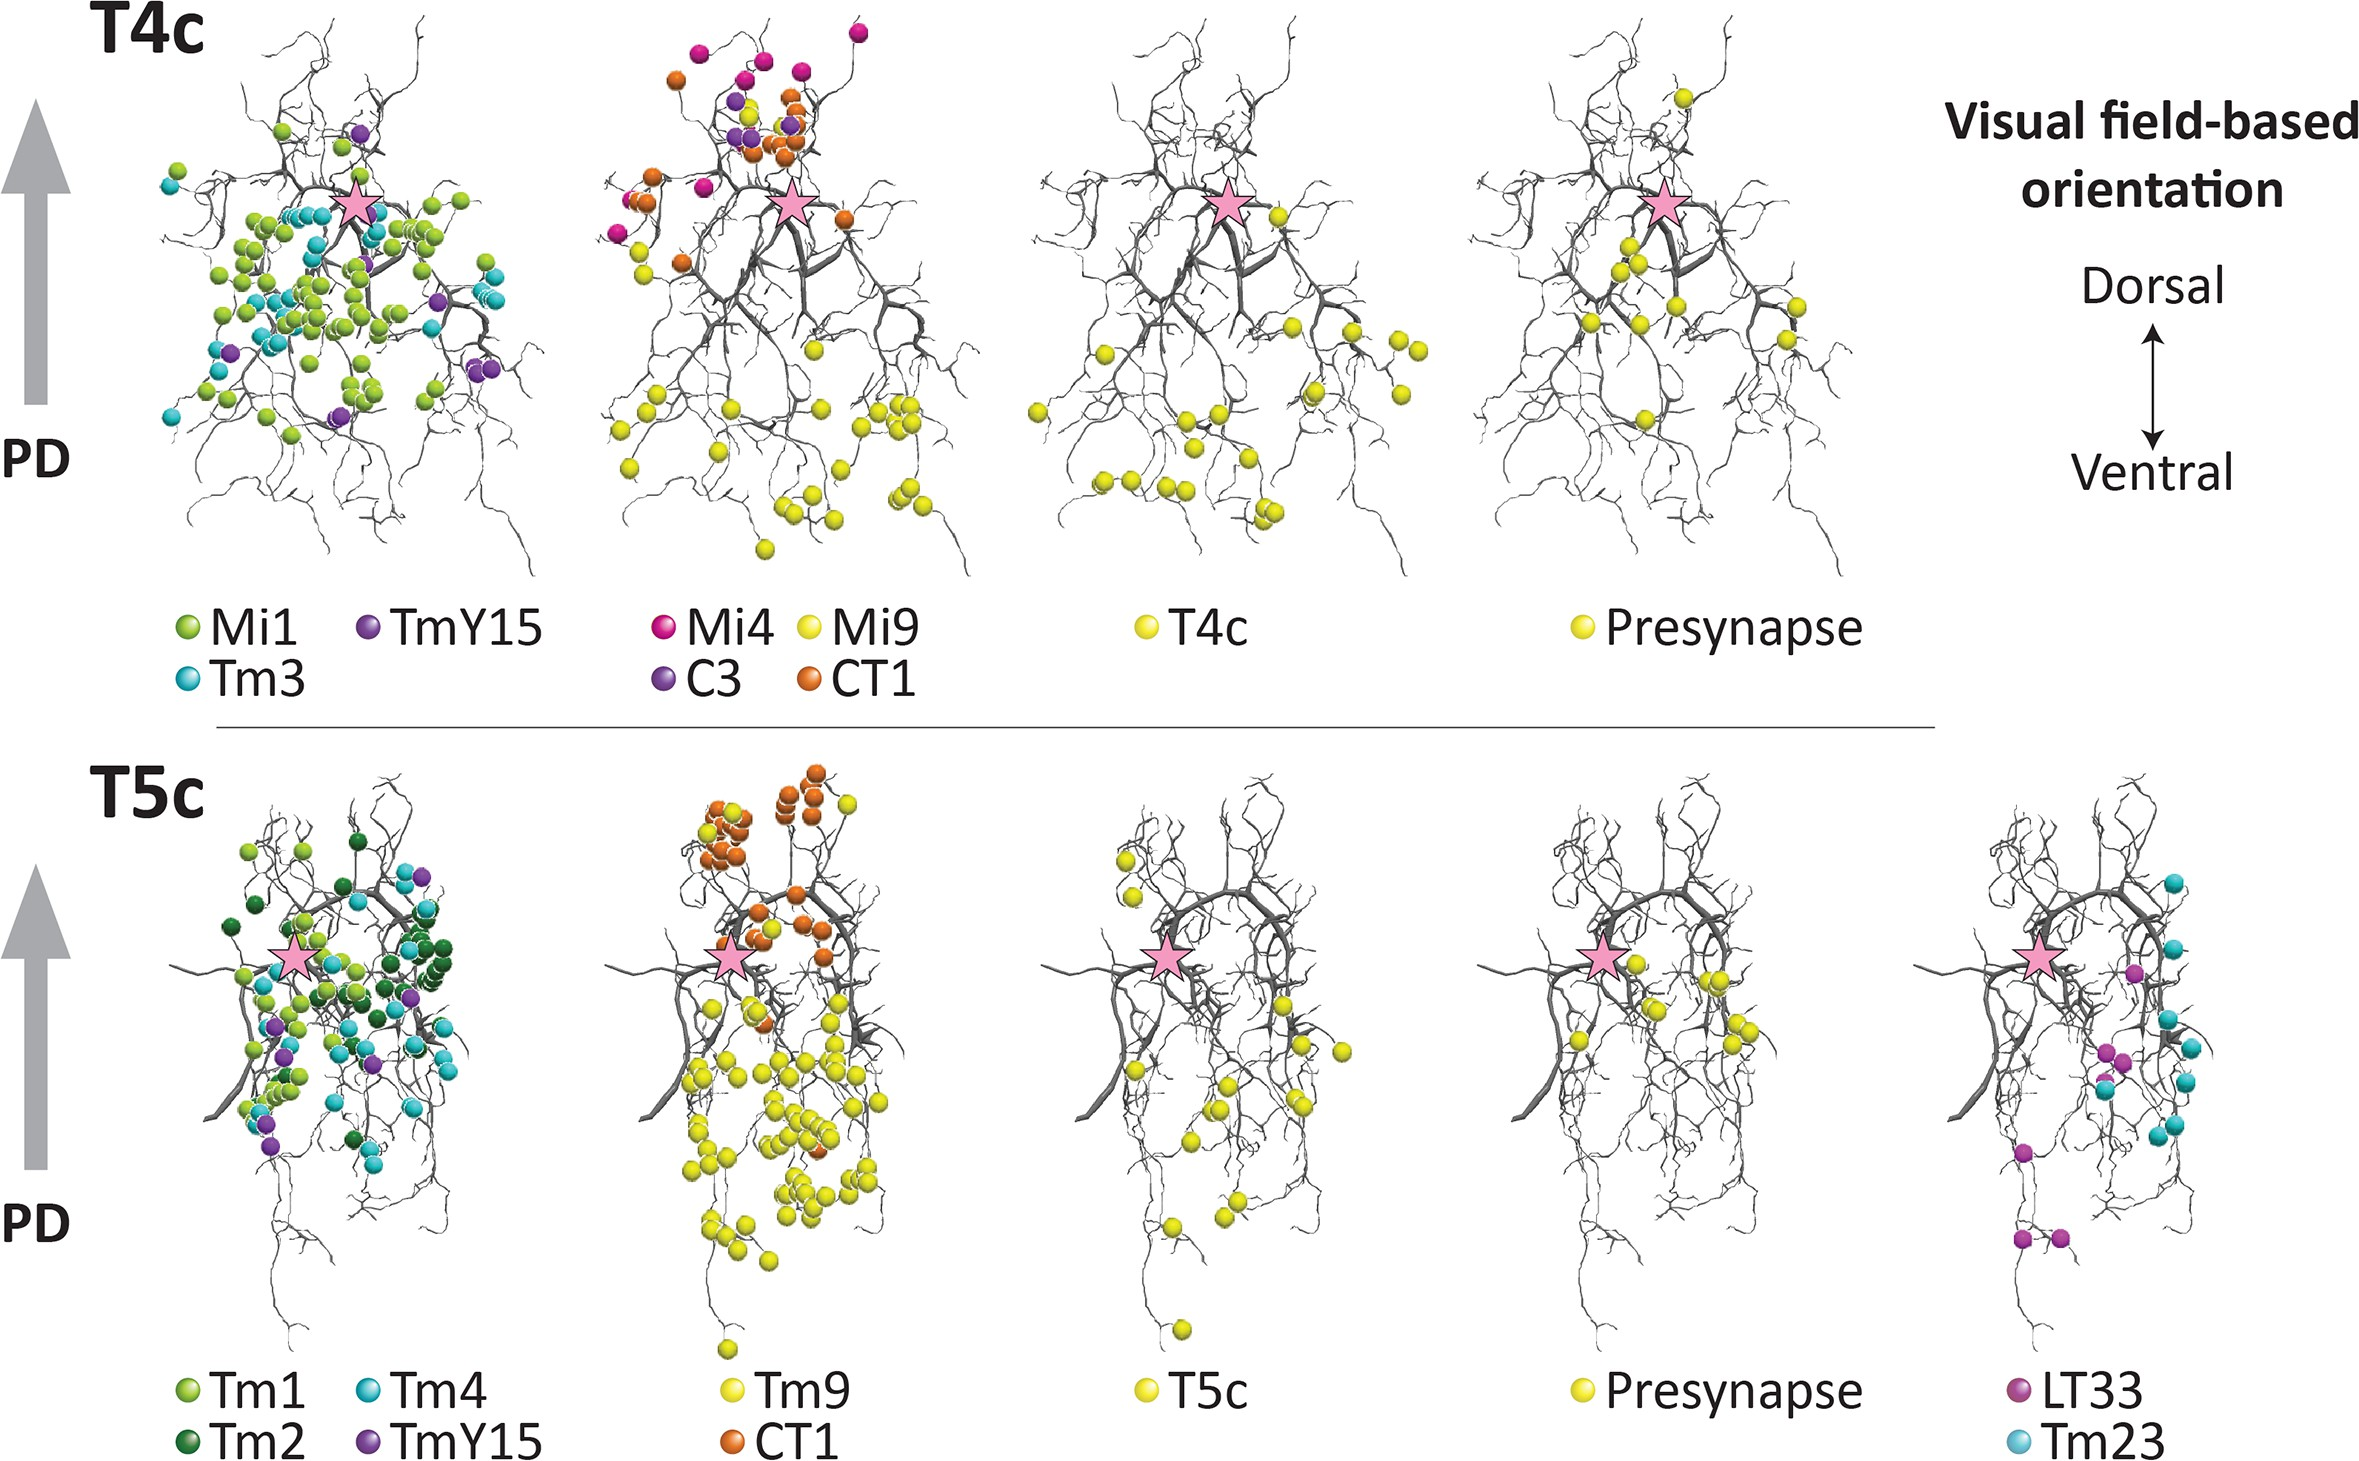
\includegraphics[scale=0.18]{t4t5inputsynapses}
\caption[Synaptic sites distributed over T4 and T5 dendritic arbors]{Synaptic sites distributed over T4 and T5 dendritic arbors: An arbor of a T4c (top panels) or T5c (bottom panels) cell is shown with synapse positions plotted on the dendritic arbors. Unless shown as 'Presynapse', puncta are postsynaptic sites (input to T4/T5 cells). T4c and T5c detect upward motion, and other subtypes of T4 and T5 cells show similar distribution patterns (not shown). An arbor's first branch point is indicated by pink stars. (Used with permission from \cite{Shinomiya2019})}
\label{fig:t4t5inputsynapses}
\end{figure}

Most of these input elements have been characterised physiologically \parencite{Arenz2017, Serbe2016, Strother2017, Meier2019, Behnia2014, Groschner2022}. None of these cells were found to be direction-selective. Hence, we can conclude that the T4 and T5 cells are the elementary motion detector found in the ON and OFF pathway respectively, and thus represents an important processing stage where the direction is computed.    

\section{Neural algorithm underlying direction selectivity}
Different models have been proposed to explain the neural computations involved in motion detection. In order to detect motion in a directionally selective manner, local motion detection mechanisms must meet certain minimum requirements \parencite{Borst1989}:
\begin{enumerate}
\item Spatial offset: Motion is a vector that needs two points to be represented, so at least two spatially separated inputs are required.
\item Temporal asymmetry: There must be at least one input that is delayed. If not, the input signals arrive in the subsequent stage simultaneously independent of the stimulus direction.
\item Non-linear interaction: It is necessary to integrate the input signals nonlinearly at a subsequent stage of the process. In the absence of this, the detector's output would be equal for both directions on average.
\end{enumerate} 

Classically two opposing models have been proposed for the implementation of direction selectivity. Both these models use two input lines, where one of the input lines has been asymmetrically delayed compared to the other, followed by a non-linear interaction. The Hassenstein-Reichardt (HR) model proposes a Preferred Direction (PD) enhancement: the signal on the preferred side is delayed and is subsequently amplified using multiplication of the signal from the other input line (figure \ref{fig:hrblmodel}a) \parencite{Hassenstein1956}. The Barlow-Levick (BL) detector, however, proposes a Null Direction (ND) suppression: the signal on the null side is delayed and divides the signal from the other input resulting in suppression (figure \ref{fig:hrblmodel}b) \parencite{Barlow1965}. \cite{Haag2016} used apparent motion stimuli to show that both the mechanisms i.e. PD enhancement on the preferred side and ND suppression on the null side are used by T4c and T5c cells to produce a direction-selective response (figure \ref{fig:hrblmodel}c). Is that special to upward-tuned T4c cells or is it general for all subtypes of T4 and T5 cells. In the first manuscript \ref{sct:manuscript_haag_mishra} - \parencite{Haag2017}, we showed that all four subtypes of T4 and T5 indeed use both PD enhancement and ND suppression to produce direction-selective responses. Therefore, a new model combining both PD enhancement on the preferred side and ND suppression on the null side was proposed. The next important task is to identify the neural correlates implementing these mechanisms. 

The model requires a fast input at the center, slow input providing excitation on the preferred side, and slow input providing suppression on the null side. Interestingly, from the anatomical and functional characterization of the input data discussed earlier, we could predict the input neurons for T4 providing these three kinds of inputs. Mi1 is a fast neuron providing input at the central part of the dendrite, thus a candidate for central fast input. Mi9 is a slow neuron providing input on the preferred side of the dendrite, hence a candidate for input on the preferred side. Mi4, C3, and CT1 are slow neurons providing input on the null side of the dendrite \parencite{Arenz2017}. 

Using two-photon voltage imaging in T5 neurons, \cite{Wienecke2018} showed that linear spatial summation is sufficient for the emergence of direction selectivity in T5 cells and that the preferred direction enhancement and null direction suppression in the calcium signal can arise from the non-linear voltage-calcium transformation. Using whole-cell recordings of T4, \cite{Gruntman2018} found that directional selectivity arises from simple integration of spatially offset fast excitatory and slow inhibitory inputs, thereby suppressing responses to nonpreferred motion directions. \cite{Groschner2022} recorded membrane potentials in T4 cells using whole-cell patch clamp recordings and in addition to the spatially offset inhibition, also found evidence for the preferred direction enhancement and a mechanism for multiplication like nonlinearity in T4 cells. In addition to synaptic mechanisms on the dendrites of T4 cells, further processing in the T4 neurons can enhance the direction selectivity of the output signals. In the second manuscript \ref{sct:manuscript_mishra_haag}, we explored the transformation of voltage to calcium in T4-cells. We found that the voltage to calcium transformation in T4c neurons enhances their direction selectivity: calcium signals in T4c cells have a significantly higher direction selectivity and tuning compared to membrane voltage across different stimuli conditions. 

\begin{figure}
\centering
\hspace*{-1cm} 
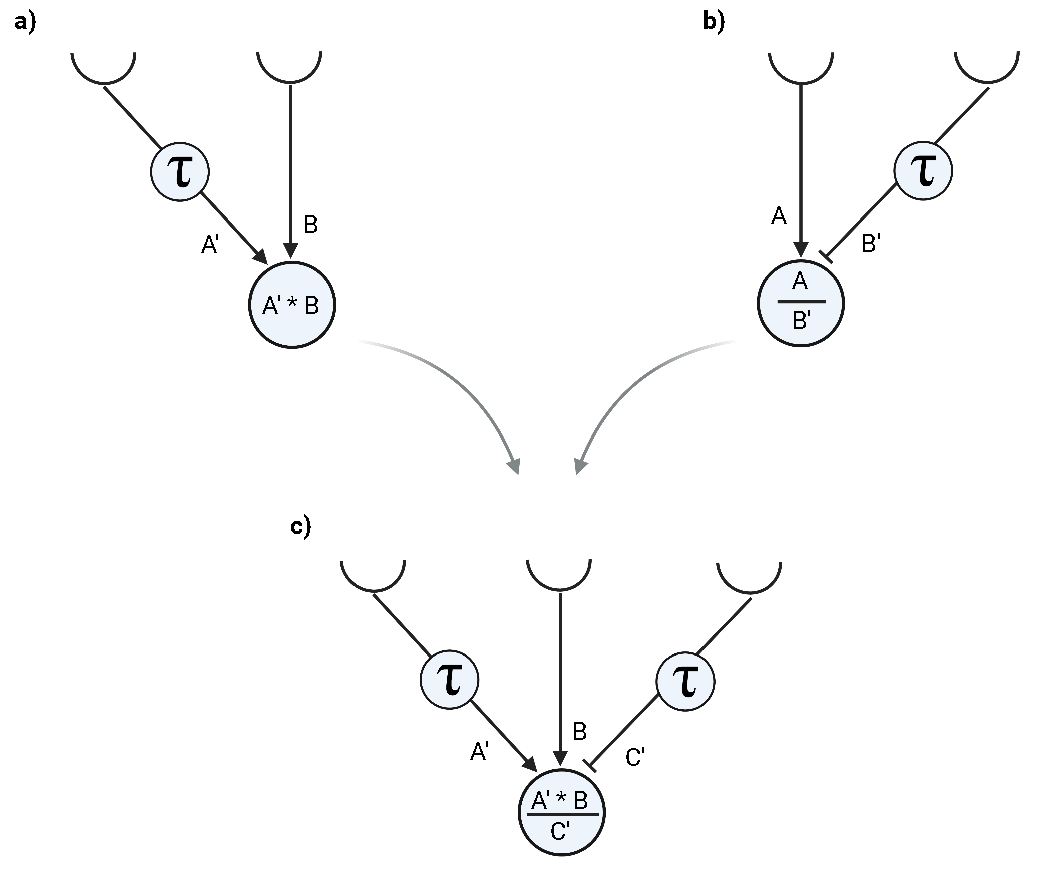
\includegraphics[scale=0.8]{HRBL_model}
\caption[Models for motion detection] {Models for motion detection: (a) The Hassenstein-Reichardt (HR) correlator (half-detector shown here) consists of two arms. Motion in the preferred direction (PD) causes two signals from neighboring photoreceptors to coincide due to a delay ($\tau$) on the first arm. There is an enhancement in PD resulting from a multiplicative non-linearity. (b) The Barlow-Levick (BL) detector has the delay on the opposite arm, and the non-linearity is inhibitory, resulting in a null-direction (ND) suppression. (c) Hybrid detector consisting of one HR unit and one BL unit: Three points in space are sampled. There is a time delay ($\tau$) on the outer two arms. The input signals from detector arms A and B are multiplied and divided by the signal from detector arm C in the following stage. Consequently, the signal in the preferred direction is enhanced and the signal in the null direction is suppressed.}
\label{fig:hrblmodel}
\end{figure}






